\documentclass[tikz,border=10pt]{standalone}
\usepackage{tikz}
\usetikzlibrary{arrows.meta, positioning, calc, shapes.geometric,
                 decorations.pathreplacing, backgrounds, fit}
\usepackage{amsmath}
\usepackage{amssymb}

\begin{document}
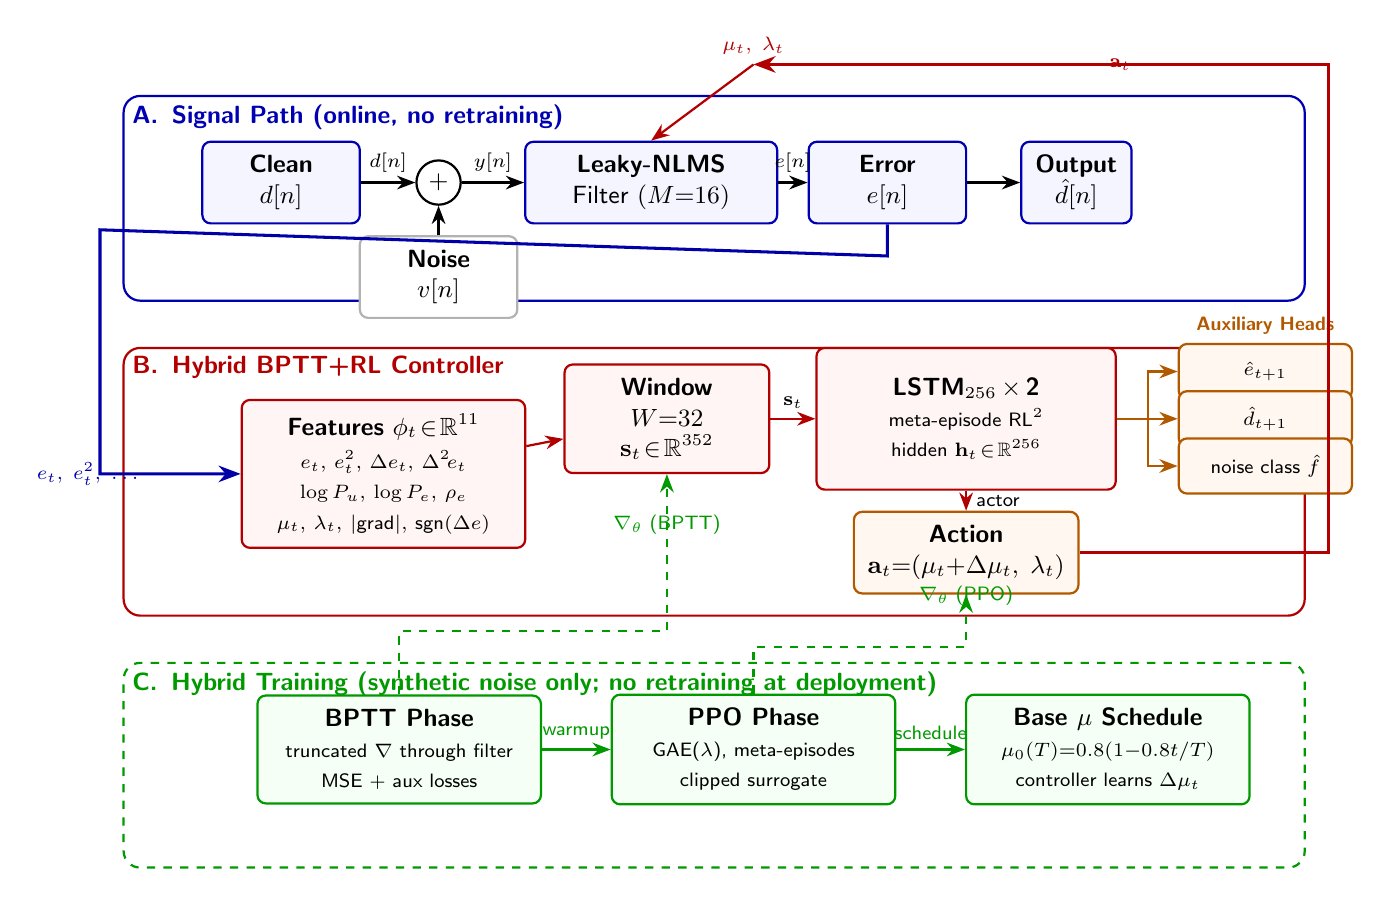
\begin{tikzpicture}[
    >=Stealth,
    font=\sffamily\small,
    box/.style={draw, thick, rounded corners=3pt, align=center,
                fill=white, inner sep=5pt,
                minimum width=2.0cm, minimum height=0.85cm},
    outerbox/.style={draw, thick, rounded corners=6pt, inner sep=10pt, fill=white},
    bluebox/.style={box, draw=blue!70!black, fill=blue!4},
    redbox/.style={box,  draw=red!70!black, fill=red!4},
    greenbox/.style={box, draw=green!60!black, fill=green!4},
    orangebox/.style={box, draw=orange!70!black, fill=orange!6},
    graybox/.style={box, draw=gray!60},
    sum/.style={circle, draw, thick, inner sep=0pt, minimum size=16pt,
                align=center, fill=white},
    arr/.style={->, thick},
    darr/.style={->, thick, dashed},
    lbl/.style={font=\sffamily\scriptsize},
]

%% ─── Box A: Signal Path ──────────────────────────────────────────────────────
\node[outerbox, draw=blue!70!black,
      minimum width=15.0cm, minimum height=2.6cm] (boxA) at (0, 7.7) {};
\node[anchor=north west, font=\sffamily\small\bfseries, text=blue!70!black]
      at (boxA.north west) {A.\enspace Signal Path (online, no retraining)};

\node[bluebox] (clean) at (-5.5, 7.9) {\textbf{Clean} \\ $d[n]$};
\node[sum]     (add)   at (-3.5, 7.9) {$+$};
\node[bluebox, minimum width=3.2cm] (filt) at (-0.8, 7.9)
      {\textbf{Leaky-NLMS} \\ Filter $(M{=}16)$};
\node[bluebox] (err)   at (2.2,  7.9) {\textbf{Error} \\ $e[n]$};
\node[graybox] (noise) at (-3.5, 6.7) {\textbf{Noise} \\ $v[n]$};
\node[bluebox, minimum width=1.4cm] (out) at (4.6, 7.9) {\textbf{Output}\\$\hat{d}[n]$};

\draw[arr] (clean) -- (add)  node[midway, above, lbl] {$d[n]$};
\draw[arr] (add)   -- (filt) node[midway, above, lbl] {$y[n]$};
\draw[arr] (filt)  -- (err)  node[midway, above, lbl] {$e[n]$};
\draw[arr] (err)   -- (out)  node[midway, above, lbl] {};
\draw[arr] (noise) -- (add);

%% mu/lambda annotation above filter
\draw[arr, draw=red!70!black, thick]
    (0.5, 9.4) -- (filt.north)
    node[pos=0, above, font=\sffamily\scriptsize, text=red!70!black]
    {$\mu_t,\;\lambda_t$};


%% ─── Box B: Hybrid Controller ────────────────────────────────────────────────
\node[outerbox, draw=red!70!black,
      minimum width=15.0cm, minimum height=3.4cm] (boxB) at (0, 4.1) {};
\node[anchor=north west, font=\sffamily\small\bfseries, text=red!70!black]
      at (boxB.north west) {B.\enspace Hybrid BPTT+RL Controller};

\node[redbox, minimum width=3.6cm, minimum height=1.8cm] (feat) at (-4.2, 4.2) {
    \textbf{Features} $\phi_t\!\in\!\mathbb{R}^{11}$\\[1pt]
    {\scriptsize $e_t,\,e_t^2,\,\Delta e_t,\,\Delta^2\!e_t$}\\
    {\scriptsize $\log P_u,\,\log P_e,\,\rho_e$}\\
    {\scriptsize $\mu_t,\,\lambda_t,\,|\text{grad}|,\,\text{sgn}(\Delta e)$}};

\node[redbox, minimum width=2.6cm] (win) at (-0.6, 4.9) {
    \textbf{Window}\\
    $W{=}32$\\
    $\mathbf{s}_t\!\in\!\mathbb{R}^{352}$};

\node[redbox, minimum width=3.8cm, minimum height=1.8cm] (lstm) at (3.2, 4.9) {
    \textbf{LSTM$_{256}$\,$\times$\,2}\\
    {\scriptsize meta-episode RL$^2$}\\
    {\scriptsize hidden $\mathbf{h}_t\!\in\!\mathbb{R}^{256}$}};

%% Action output
\node[orangebox, minimum width=2.0cm] (action) at (3.2, 3.2) {
    \textbf{Action}\\
    $\mathbf{a}_t{=}(\mu_t{+}\Delta\mu_t,\;\lambda_t)$};

%% Auxiliary heads (to the right)
\node[orangebox, minimum width=2.2cm, minimum height=0.7cm] (herr) at (7.0, 5.5) {
    {\scriptsize $\hat{e}_{t+1}$}};
\node[orangebox, minimum width=2.2cm, minimum height=0.7cm] (hsig) at (7.0, 4.9) {
    {\scriptsize $\hat{d}_{t+1}$}};
\node[orangebox, minimum width=2.2cm, minimum height=0.7cm] (htask) at (7.0, 4.3) {
    {\scriptsize noise class $\hat{f}$}};

\node[font=\sffamily\scriptsize\bfseries, text=orange!70!black, anchor=south]
    at (7.0, 5.85) {Auxiliary Heads};

\draw[arr, draw=red!70!black] (feat)  -- (win)   node[midway, above, lbl] {};
\draw[arr, draw=red!70!black] (win)   -- (lstm)  node[midway, above, lbl] {$\mathbf{s}_t$};
\draw[arr, draw=red!70!black] (lstm)  -- (action) node[midway, right, lbl] {actor};
\draw[draw=orange!70!black, thick] (lstm.east) -- ++(0.4, 0) coordinate (fork);
\draw[arr, draw=orange!70!black] (fork) |- (herr.west);
\draw[arr, draw=orange!70!black] (fork) |- (hsig.west);
\draw[arr, draw=orange!70!black] (fork) |- (htask.west);


%% ─── Box C: Hybrid Training ──────────────────────────────────────────────────
\node[outerbox, draw=green!60!black, dashed,
      minimum width=15.0cm, minimum height=2.6cm] (boxC) at (0, 0.5) {};
\node[anchor=north west, font=\sffamily\small\bfseries, text=green!60!black]
      at (boxC.north west)
      {C.\enspace Hybrid Training (synthetic noise only; no retraining at deployment)};

\node[greenbox, minimum width=3.6cm] (bptt) at (-4.0, 0.7) {
    \textbf{BPTT Phase}\\
    {\scriptsize truncated $\nabla$ through filter}\\
    {\scriptsize MSE + aux losses}};

\node[greenbox, minimum width=3.6cm] (rl) at (0.5, 0.7) {
    \textbf{PPO Phase}\\
    {\scriptsize GAE($\lambda$), meta-episodes}\\
    {\scriptsize clipped surrogate}};

\node[greenbox, minimum width=3.6cm] (sched) at (5.0, 0.7) {
    \textbf{Base $\mu$ Schedule}\\
    {\scriptsize $\mu_0(T){=}0.8(1{-}0.8t/T)$}\\
    {\scriptsize controller learns $\Delta\mu_t$}};

\draw[arr, draw=green!60!black] (bptt) -- (rl)
    node[midway, above, lbl, text=green!60!black] {warmup};
\draw[arr, draw=green!60!black] (rl) -- (sched)
    node[midway, above, lbl, text=green!60!black] {schedule};


%% ─── Inter-box connections ────────────────────────────────────────────────────

%% e[n] → Features (left side, counter-clockwise)
\draw[arr, draw=blue!65!black, line width=1.1pt]
    (err.south) -- ++(0, -0.4)
    -- (-7.8, 7.3)
    -- (-7.8, 4.2)
    -- (feat.west)
    node[pos=0.35, left, lbl, text=blue!65!black] {$e_t,\;e_t^2,\;\ldots$};

%% Action → Filter (right side, clockwise)
\draw[arr, draw=red!70!black, line width=1.1pt]
    (action.east) -- (7.8, 3.2)
    -- (7.8, 9.4)
    -- (0.5, 9.4)
    node[pos=0.4, right, lbl, text=red!70!black] {$\mathbf{a}_t$};

%% BPTT gradient (dashed green)
\draw[darr, draw=green!60!black]
    (bptt.north) -- (-4.0, 2.2) -- (-0.6, 2.2) -- (win.south)
    node[pos=0.55, above, lbl, text=green!60!black] {$\nabla_\theta$ (BPTT)};

%% PPO gradient (dashed green)
\draw[darr, draw=green!60!black]
    (rl.north) -- (0.5, 2.0) -- (3.2, 2.0) -- (action.south)
    node[pos=0.6, above, lbl, text=green!60!black] {$\nabla_\theta$ (PPO)};

\end{tikzpicture}
\end{document}
